\documentclass[conference]{IEEEtran}
\IEEEoverridecommandlockouts
% The preceding line is only needed to identify funding in the first footnote. If that is unneeded, please comment it out.
\usepackage{cite}
\usepackage{amsmath,amssymb,amsfonts}
\usepackage{algorithmic}
\usepackage{graphicx}
\usepackage{textcomp}
\usepackage{xcolor}
\usepackage{url}
\usepackage{hyperref}
\def\BibTeX{{\rm B\kern-.05em{\sc i\kern-.025em b}\kern-.08em
    T\kern-.1667em\lower.7ex\hbox{E}\kern-.125emX}}
\begin{document}

\title{Developing a DVB-I Parser Library in Dart and GUI App in Flutter\\}

\author{\IEEEauthorblockN{1\textsuperscript{st} Luis Hebendanz}
\IEEEauthorblockA{\textit{M. Sc. Computer Science}\\
\textit{TU Berlin}\\
Berlin, Germany \\}
\and
\IEEEauthorblockN{2\textsuperscript{nd} Nicklas}
\IEEEauthorblockA{\textit{M. Sc. Information Systems Management} \\
\textit{TU Berlin}\\
Berlin, Germany \\}
\and
\IEEEauthorblockN{3\textsuperscript{rd} Balint}
\IEEEauthorblockA{\textit{M. Sc. Information Systems Management} \\
	\textit{TU Berlin}\\
	Berlin, Germany \\}
\and

}

\maketitle

\begin{abstract}
 In this project, we aimed to develop an efficient DVB-I parser library in Dart and a GUI app in Flutter to present TV services on Android devices.

We used the Dart programming language to write the DVB-I parser library and Google's cross-platform Flutter framework to develop the GUI app.

 However, we faced challenges in developing the GUI app in Flutter due to multiple bugs in the libraries we used and sparse documentation. Despite these challenges, we were able to develop a working app to present TV services on Android devices.

Our project demonstrates the feasibility of using Dart to write an efficient DVB-I parser library and Flutter to develop a GUI app that presents TV services on Android devices. However the challenges we faced in developing the GUI app highlight the importance of mature libraries and documentation to support developers in using these technologies. The lack of maturity in the Flutter ecosystem has compelled us to not recommend it for further projects.
\end{abstract}

\begin{IEEEkeywords}
IP-TV, DVB-I, Flutter, Dart, Cross Platform
\end{IEEEkeywords}

\section{Introduction}
In this project, we aimed to develop an efficient DVB-I parser library in Dart and a GUI app in Flutter to present TV services on Android devices. The DVB-I standard is a standards-based solution for delivering television via the internet and offers a discovery mechanism to signal and discover television services, using a set of REST APIs allowing clients to retrieve a list of services in an XML-based format. Our primary objective was to create a parser library that can efficiently handle the DVB-I service list registry and provide all the necessary information required to present the TV service in the client app. Additionally, we aimed to create an Android GUI app using Flutter that uses the DVB-I parser library to present the TV services to the user. 

The development of the DVB-I parser library involved reading the DVB-I standard and manually emulating REST requests as specified by the specification. We also familiarized ourselves with the Dart programming language and experimented with simple coding examples to gain proficiency with the language. Once we had a good understanding of the standard and the language, we designed and developed the DVB-I parser library using Dart, implementing the required REST APIs and XML parsing. 

The development of the Android GUI app using Flutter involved building an intuitive user interface to present the TV services to the user, as well as incorporating the DVB-I parser library to retrieve and display the information for each service. We faced challenges while developing the app, including multiple bugs in libraries used and sparse documentation, which affected the app's functionality and usability.

In this evaluation, we will assess the success of our project in achieving its goals and evaluate the performance and usability of the DVB-I parser library and Android GUI app developed. We will also discuss the challenges encountered during development and recommend future improvements to enhance the overall functionality and usability of the app.

\section{Scientific Background}

In this section we will go over the technologies used and their functionality. 

\subsection{DVB-I Standard}





\subsection{Flutter Framework}\label{AA}

\section{Architecture Overview}

Flutter is a cross-platform framework for building mobile and desktop applications. Its architecture consists of four main layers: the Dart app layer, the framework layer, the engine layer, and the platform layer. Shown in figure \ref{fig:flutter_tech_stack}.

\begin{figure}[ht]
	\centerline{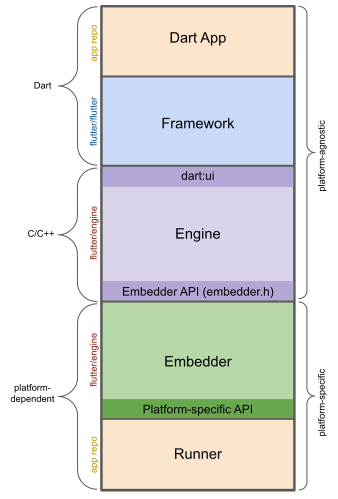
\includegraphics[width=\linewidth]{figures/app-anatomy}}
	\caption{Flutter architectural overview \cite{b1.1}}
	\label{fig:flutter_tech_stack}
\end{figure}

The Dart app layer is responsible for composing widgets into the desired UI and implementing business logic. It is owned by the app developer.

The framework layer provides a higher-level API for building UI apps, including widgets, hit-testing, gesture detection, accessibility, and text input. It composites the app's widget tree into a scene.

The engine layer is responsible for rasterizing composited scenes and provides low-level implementation of Flutter's core APIs, including graphics, text layout, and the Dart runtime. It exposes its functionality to the framework using the dart:ui API and integrates with a specific platform using the platform layer.

The platform layer ``is the native OS application that hosts all Flutter content and acts as the glue between the host operating system and Flutter``\cite{b1.1}. Flutter includes platform embedders for each of the target platforms, and you can also create a custom platform embedder.

In summary, Flutter's architecture provides a robust and efficient rendering pipeline, bypassing system UI widget libraries and using its own widget set and Skia 2D library for rendering. This results in a high-performance, cross-platform framework with minimal abstractions and overhead.

\section{Integrating with other code}



\subsection{Units}

\section{Theoretical Background}

\subsection{DVB-I Standard}

%DVB-I standard rough overview of the structure

%What is DVBI


The DVB-I (DVB-Internet) standard is a specification developed by the Digital Video Broadcasting (DVB) organization for delivering linear television services over the internet.The standard defines the mechanisms to be used to find sets of linear television services delivered through broadband or broadcast mechanisms as well as methods to retrieve electronic programme data for those services.[ref to document]

The core of the specification is the Service List Registry (SLR) which provides a set of REST APIs allowing clients (TVs, Mobile, Browser) to retrieve a list of services (ServiceList) in an XML-based format including all information required to present the TV service in the client. The DVB-I standard, published by ETSI, expands upon the existing DVB Broadcast-based delivery methods, such as Terrestrial, Satellite, and Cable, to provide simpler and more accessible options for viewing both Linear and VOD Streaming services on any internet-connected device. With this open standard, users can enjoy a seamless viewing experience across multiple devices without any limitations.






\subsection{Flutter}



What is Flutter. How does it work? Why we chose it?

Flutter is an open-source mobile app development framework developed by Google that allows developers to create high-performance, cross-platform mobile applications for iOS, Android, and other platforms from a single codebase.

Flutter uses a programming language called Dart, which is also developed by Google, and provides a rich set of pre-built UI widgets and tools that allow developers to create visually appealing and interactive mobile applications. The framework uses a reactive programming model, which means that changes in the app's state are automatically reflected in the UI, making it easy to build dynamic user interfaces.

One of the key benefits of Flutter is its hot-reload feature, which allows developers to quickly see the changes they make to the code in real-time on the app, without having to rebuild the entire application. This significantly speeds up the development process and makes it easier for developers to experiment with different UI designs and functionality.

Flutter is also known for its fast development speed and ease of use, making it an ideal choice for startups and businesses that need to quickly develop and deploy high-quality mobile applications.

In addition to mobile app development, Flutter can also be used for building desktop and web applications, thanks to its platform-independent nature. Overall, Flutter is a powerful and flexible mobile app development framework that is rapidly gaining popularity in the developer community.


\section{Implementation}



Our implementation is split into four big parts: the development setup \ref{dev_set}, a general overview of the architcture  \ref{arch}, the dvb-i parser libary, which contains all the xml parsings and http requests \ref{dvbi_parser} and finally the user interface which the client interacts with. \ref{gui}. The code for this implementation can be found on \emph{github}\footnote{\url{https://github.com/AWT-DVBI/dvbi_client}}.


\subsection{Development Setup}\label{dev_set}

Development Setup:
Using Nix for a development environment
TODO: Setup for Windows
describe important libs that were used


\subsection{Architecture}\label{arch}

\subsubsection{General Overview}
General Architecture:
walkthrough of how a user interacts with client and how parser requests more info
graphic of architecture


\subsection{Dvb-I Parser}\label{dvbi_parser}

libraries used
XML to Dart object mapping
Features:
Lazy loading. Only request data you need. Request more on obj access
Async http request for parallel fetching
XML to JSON parsing  

\subsection{Gui Application}\label{gui}

libraries used(?)
layout of GUI/Screenshots
Content Guide Page
features: breaks everything 
Channel Browsing
features: subtitles, volume control, next/prev channel, show channel logo and name

\section{Challenges}

Dart Streams, Dart async
idea: reduce loading times by asynchr loading channels. 
State Management in Flutter: 
Unaccounted for Dart language features in Riverpod
Riverpod: Providers + Dart streams = StreamProviders
out-of-the-box state management using State widgets
	
DVB-I Server wrong response data with official endpoints ( use of different staging Endpoints for correct data)
start and end time 
flexibility in standard leads to many edge cases 
Bugs in libraries: videoplayer, chewie
o(n2) performance issue due to the structure of the given xml tree and our used xml lib

\section{Evaluation}

scalability
include screenshots cross platform framework flutter ....does it work on android and apples ios?
only android in combination with exoplayer as mpeg dash is not supported by hls and the current flutter videoplayer libs

\section{Conclusion and Future Work}

subtitles, channel info button



\subsection{Figures and Tables}
\paragraph{Positioning Figures and Tables} Place figures and tables at the top and 
bottom of columns. Avoid placing them in the middle of columns. Large 
figures and tables may span across both columns. Figure captions should be 
below the figures; table heads should appear above the tables. Insert 
figures and tables after they are cited in the text. Use the abbreviation 
``Fig.~\ref{fig}'', even at the beginning of a sentence.

\begin{table}[htbp]
\caption{Table Type Styles}
\begin{center}
\begin{tabular}{|c|c|c|c|}
\hline
\textbf{Table}&\multicolumn{3}{|c|}{\textbf{Table Column Head}} \\
\cline{2-4} 
\textbf{Head} & \textbf{\textit{Table column subhead}}& \textbf{\textit{Subhead}}& \textbf{\textit{Subhead}} \\
\hline
copy& More table copy$^{\mathrm{a}}$& &  \\
\hline
\multicolumn{4}{l}{$^{\mathrm{a}}$Sample of a Table footnote.}
\end{tabular}
\label{tab1}
\end{center}
\end{table}

\begin{figure}[htbp]
\centerline{
\includegraphics{fig1.png}}
\caption{Example of a figure caption.}
\label{fig}
\end{figure}

Figure Labels: Use 8 point Times New Roman for Figure labels. Use words 
rather than symbols or abbreviations when writing Figure axis labels to 
avoid confusing the reader. As an example, write the quantity 
``Magnetization'', or ``Magnetization, M'', not just ``M''. If including 
units in the label, present them within parentheses. Do not label axes only 
with units. In the example, write ``Magnetization (A/m)'' or ``Magnetization 
\{A[m(1)]\}'', not just ``A/m''. Do not label axes with a ratio of 
quantities and units. For example, write ``Temperature (K)'', not 
``Temperature/K''.

\section*{Acknowledgment}

The preferred spelling of the word ``acknowledgment'' in America is without 
an ``e'' after the ``g''. Avoid the stilted expression ``one of us (R. B. 
G.) thanks $\ldots$''. Instead, try ``R. B. G. thanks$\ldots$''. Put sponsor 
acknowledgments in the unnumbered footnote on the first page.

\section*{References}

Please number citations consecutively within brackets \cite{b1}. The 
sentence punctuation follows the bracket \cite{b2}. Refer simply to the reference 
number, as in \cite{b3}---do not use ``Ref. \cite{b3}'' or ``reference \cite{b3}'' except at 
the beginning of a sentence: ``Reference \cite{b3} was the first $\ldots$''

Number footnotes separately in superscripts. Place the actual footnote at 
the bottom of the column in which it was cited. Do not put footnotes in the 
abstract or reference list. Use letters for table footnotes.

Unless there are six authors or more give all authors' names; do not use 
``et al.''. Papers that have not been published, even if they have been 
submitted for publication, should be cited as ``unpublished'' \cite{b4}. Papers 
that have been accepted for publication should be cited as ``in press'' \cite{b5}. 
Capitalize only the first word in a paper title, except for proper nouns and 
element symbols.

For papers published in translation journals, please give the English 
citation first, followed by the original foreign-language citation \cite{b6}.

\begin{thebibliography}{00}
\bibitem{b1.1} Flutter, ``Flutter architectural overview``, [Online] \url{https://docs.flutter.dev/resources/architectural-overview}
	
%=============================0%
\bibitem{b1} G. Eason, B. Noble, and I. N. Sneddon, ``On certain integrals of Lipschitz-Hankel type involving products of Bessel functions,'' Phil. Trans. Roy. Soc. London, vol. A247, pp. 529--551, April 1955.
\bibitem{b2} J. Clerk Maxwell, A Treatise on Electricity and Magnetism, 3rd ed., vol. 2. Oxford: Clarendon, 1892, pp.68--73.
\bibitem{b3} I. S. Jacobs and C. P. Bean, ``Fine particles, thin films and exchange anisotropy,'' in Magnetism, vol. III, G. T. Rado and H. Suhl, Eds. New York: Academic, 1963, pp. 271--350.
\bibitem{b4} K. Elissa, ``Title of paper if known,'' unpublished.
\bibitem{b5} R. Nicole, ``Title of paper with only first word capitalized,'' J. Name Stand. Abbrev., in press.
\bibitem{b6} Y. Yorozu, M. Hirano, K. Oka, and Y. Tagawa, ``Electron spectroscopy studies on magneto-optical media and plastic substrate interface,'' IEEE Transl. J. Magn. Japan, vol. 2, pp. 740--741, August 1987 [Digests 9th Annual Conf. Magnetics Japan, p. 301, 1982].
\bibitem{b7} M. Young, The Technical Writer's Handbook. Mill Valley, CA: University Science, 1989.
\end{thebibliography}
\vspace{12pt}
\color{red}
IEEE conference templates contain guidance text for composing and formatting conference papers. Please ensure that all template text is removed from your conference paper prior to submission to the conference. Failure to remove the template text from your paper may result in your paper not being published.

\end{document}
